\documentclass[compress]{beamer}
\usetheme{sthlm}

%-=-=-=-=-=-=-=-=-=-=-=-=-=-=-=-=-=-=-=-=-=-=-=-=
%        LOADING BEAMER PACKAGES
%-=-=-=-=-=-=-=-=-=-=-=-=-=-=-=-=-=-=-=-=-=-=-=-=

\usepackage{
booktabs,
datetime,
dtk-logos,
graphicx,
multicol,
pgfplots,
ragged2e,
tabularx,
tikz,
wasysym,
multirow,
float,
caption,
subcaption
}

\pgfplotsset{compat=1.8}

\usepackage[utf8]{inputenc}
\usepackage[portuguese]{babel}
\usepackage[T1]{fontenc}
\usepackage{newpxtext,newpxmath}
\usepackage{listings}

\lstset{ %
language=[LaTeX]TeX,
basicstyle=\normalsize\ttfamily,
keywordstyle=,
numbers=left,
numberstyle=\tiny\ttfamily,
stepnumber=1,
showspaces=false,
showstringspaces=false,
showtabs=false,
breaklines=true,
frame=tb,
framerule=0.5pt,
tabsize=4,
framexleftmargin=0.5em,
framexrightmargin=0.5em,
xleftmargin=0.5em,
xrightmargin=0.5em
}



%-=-=-=-=-=-=-=-=-=-=-=-=-=-=-=-=-=-=-=-=-=-=-=-=
%        LOADING TIKZ LIBRARIES
%-=-=-=-=-=-=-=-=-=-=-=-=-=-=-=-=-=-=-=-=-=-=-=-=

\usetikzlibrary{
backgrounds,
mindmap
}

%-=-=-=-=-=-=-=-=-=-=-=-=-=-=-=-=-=-=-=-=-=-=-=-=
%        BEAMER OPTIONS
%-=-=-=-=-=-=-=-=-=-=-=-=-=-=-=-=-=-=-=-=-=-=-=-=

\setbeameroption{show notes}

%-=-=-=-=-=-=-=-=-=-=-=-=-=-=-=-=-=-=-=-=-=-=-=-=
%        BEAMER COMMANDS
%-=-=-=-=-=-=-=-=-=-=-=-=-=-=-=-=-=-=-=-=-=-=-=-=


%-=-=-=-=-=-=-=-=-=-=-=-=-=-=-=-=-=-=-=-=-=-=-=-=
%
%	PRESENTATION INFORMATION
%
%-=-=-=-=-=-=-=-=-=-=-=-=-=-=-=-=-=-=-=-=-=-=-=-=

\title{Fundamentos de \\ comunicação entre \\ processos}
\subtitle{DCE540 - Computação Paralela e Distribuída}
%\date{\small{\jobname}}
\author{\texttt{Iago Carvalho}}
\institute{\texttt{Departamento de Ciência da Computação}}

\hypersetup{
pdfauthor = {Iago A. Carvalho},      
pdfsubject = {Computação Paralela e Distribuída},
pdfkeywords = {},  
pdfmoddate= {D:\pdfdate},          
pdfcreator = {WriteLaTeX}
}

\begin{document}

\begin{frame}
\titlepage

\end{frame}

%% --------------------------------------------------------

\begin{frame}{Comunicação}

Em sistemas computacionais não distribuídos, comunicação entre processos é uma tarefa bem simples
\begin{itemize}
    \item Arquivos
    \item Memória compartilhada
\end{itemize}

Entretanto, quando temos diversos dispositivos espalhados por todo o mundo, esta tarefa é um pouco mais complicada...
\begin{itemize}
    \item Baseada em protocolos de baixo nível
    \item Troca de mensagens
    \item Remote Procedure Calls (RPC)
\end{itemize}

\end{frame}


%% --------------------------------------------------------

\begin{frame}{Modelo OSI}

Para começarmos a discutir os processos de comunicação, devemos primeiro entender o modelo OSI \href{https://pt.wikipedia.org/wiki/Modelo_OSI}{\beamergotobutton{Link}} 
\begin{itemize}
    \item ISO \textbf{O}pen \textbf{S}ystems \textbf{I}nterconnection Reference Model
\end{itemize}

\vspace{0.5cm}

O modelo OSI é dividido em 7 camadas
\begin{itemize}
    \item Cada camada com diversos protocolos de comunicação
    \item Em geral, protocolos são \textit{mortos}
\end{itemize}

\vspace{0.5cm}

A grande vantagem do modelo OSI é auxiliar no entendimento de como redes de computadores funcionam
\end{frame}

%% --------------------------------------------------------

\begin{frame}{Modelo OSI}

\vspace{0.3cm}

\centering 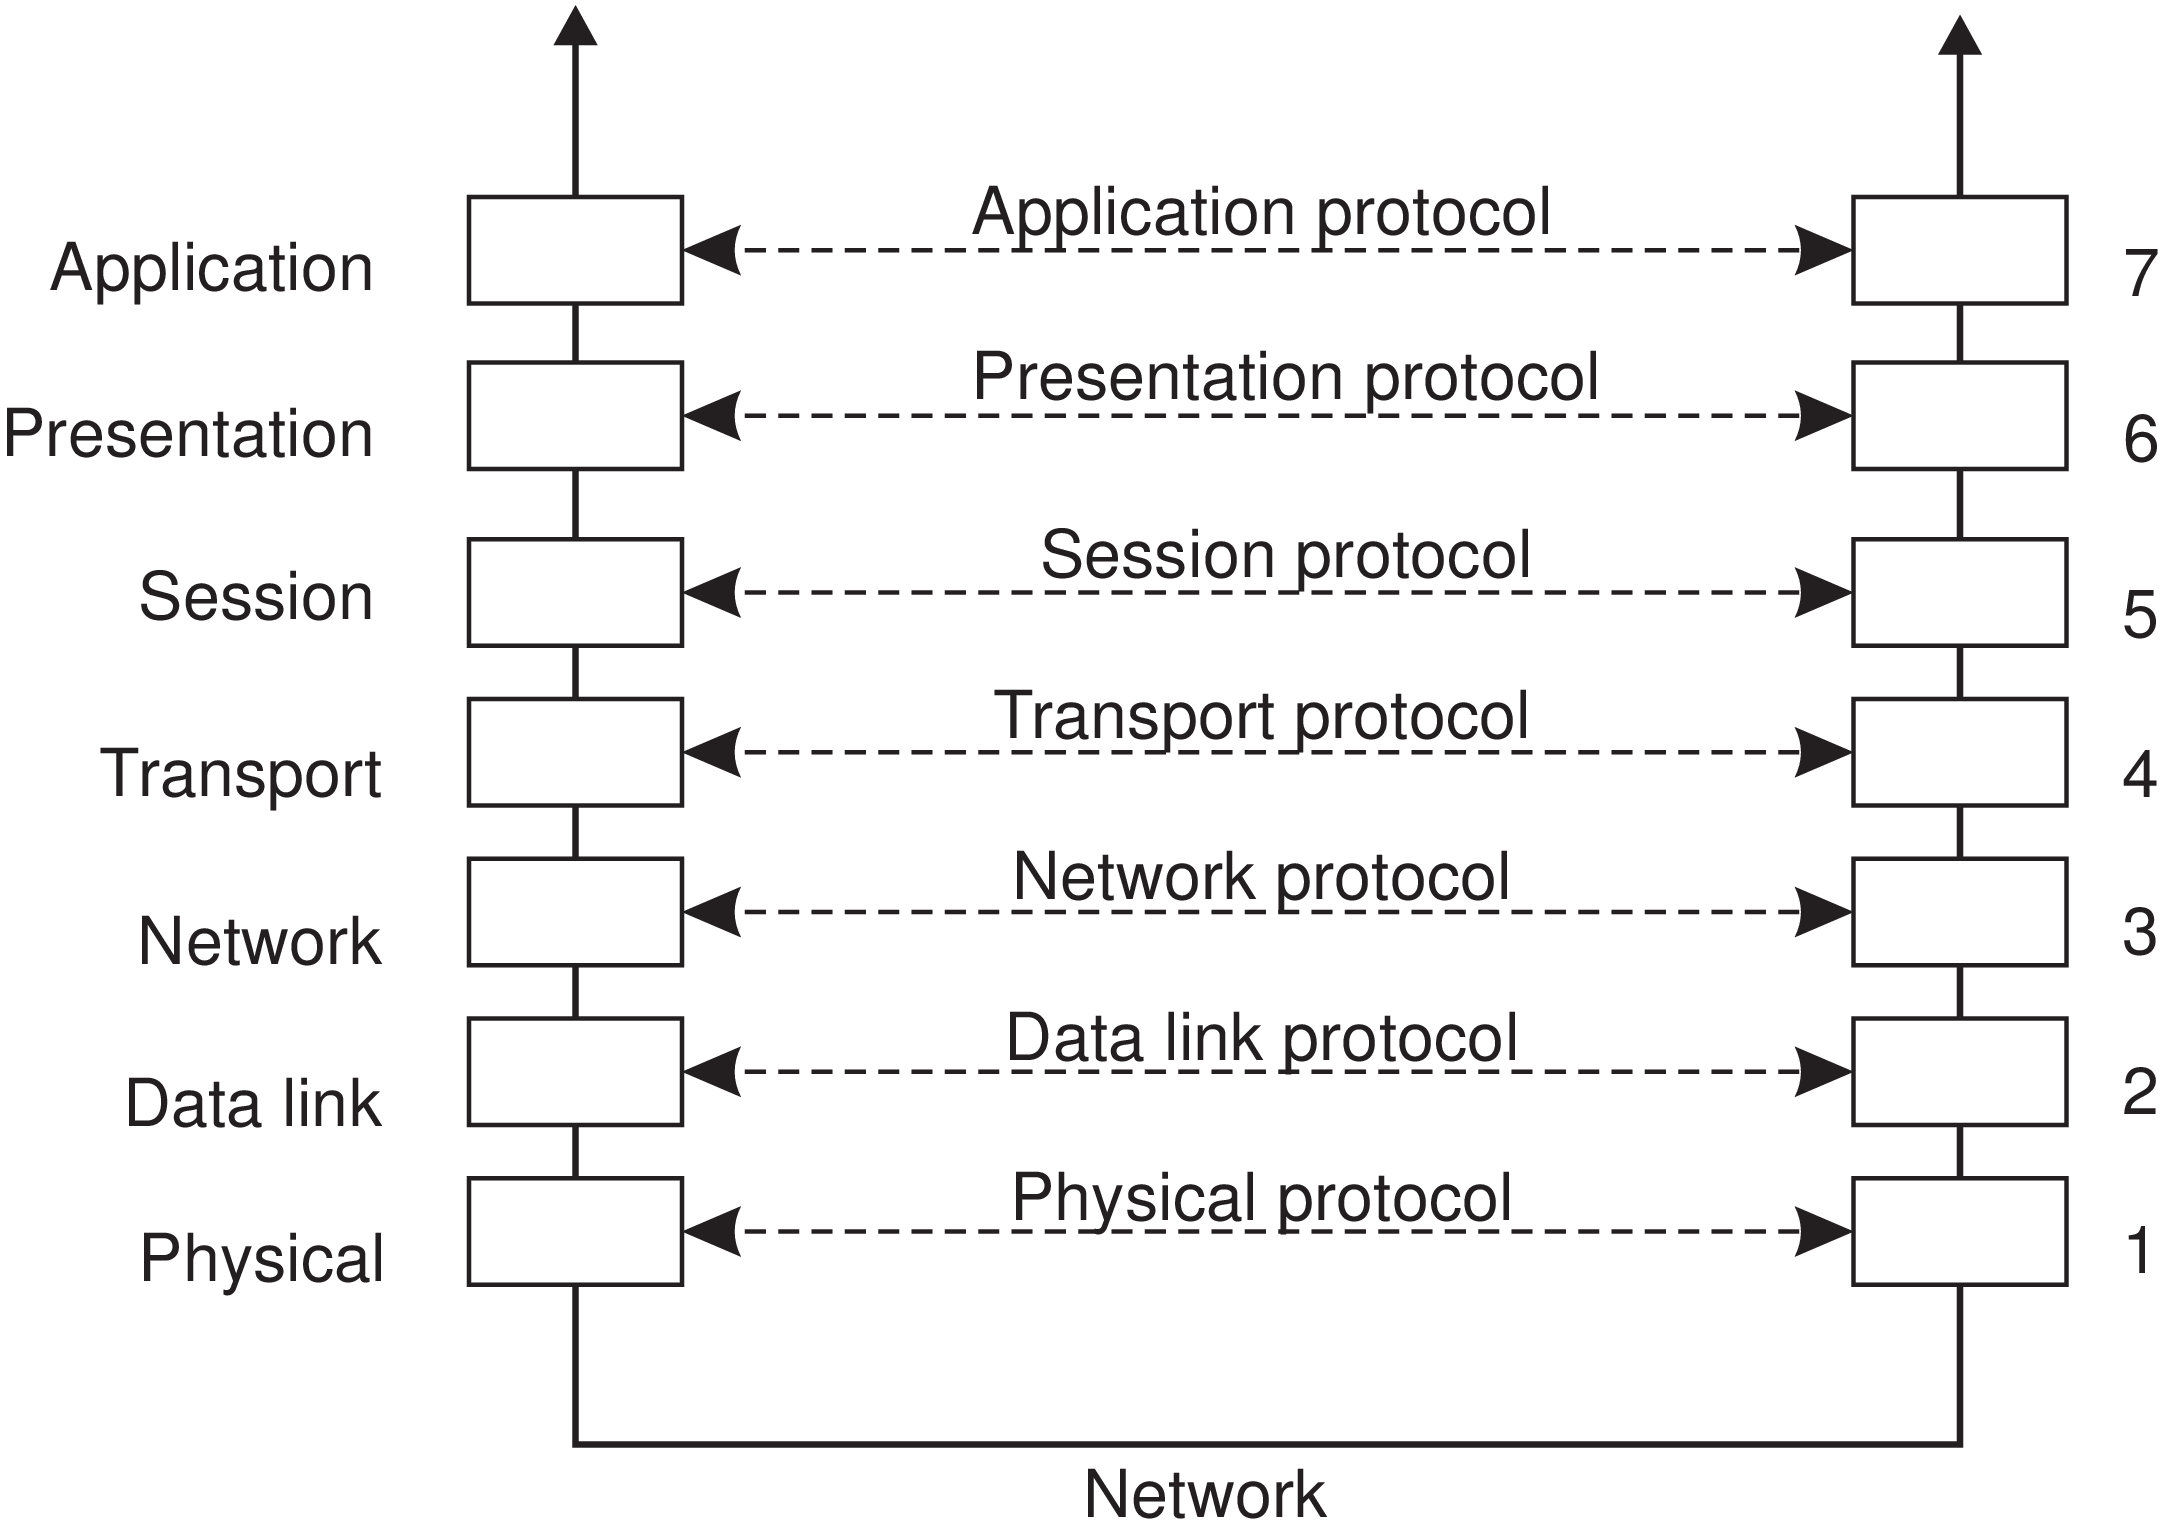
\includegraphics[width=0.95\textwidth]{images/osi.png}

\end{frame}

%% --------------------------------------------------------

\begin{frame}{Camadas no modelo OSI}

Camada de aplicação
\begin{itemize}
    \item A aplicação, literalmente
    \item E-mail, transferência de arquivos,  web...
\end{itemize}

Camada de apresentação
\begin{itemize}
    \item Controla a maneira como os dados são representados
    \item Tradução de dados
    \item Criptografia e segurança
\end{itemize}

Camada de sessão (\textit{data link})
\begin{itemize}
    \item Estabelece a comunicação entre duas aplicações
\end{itemize}

Camada de transporte
\begin{itemize}
    \item Protocolos de comunicação entre aplicações
    \begin{itemize}
        \item Confiáveis ou não
    \end{itemize}
\end{itemize}

\end{frame}

%% --------------------------------------------------------

\begin{frame}{Camadas no modelo OSI}

Camada de rede
\begin{itemize}
    \item Controla o fluxo de mensagens na rede
    \item Roteamento de mensagens
    \item Prevenção e tratamento de congestionamento 
\end{itemize}

\vspace{0.5cm}

Camada de enlace (\textit{data link})
\begin{itemize}
    \item Detecção e correção de erros de transmissão
\end{itemize}

\vspace{0.5cm}

Camada física
\begin{itemize}
    \item Como os computadores estão conectados entre si
    \begin{itemize}
        \item Cabos
        \item Wi-Fi
        \item $\ldots$
    \end{itemize}
    \item Representação binária dos dados
\end{itemize}

\end{frame}

%% --------------------------------------------------------

\begin{frame}{Mensagem de rede}

Processo \textbf{P} quer se comunicar com um processo remoto \textbf{Q}
\begin{itemize}
    \item \textbf{P} tem que enviar uma mensagem para \textbf{Q}
\end{itemize}

\vspace{1cm}

\centering 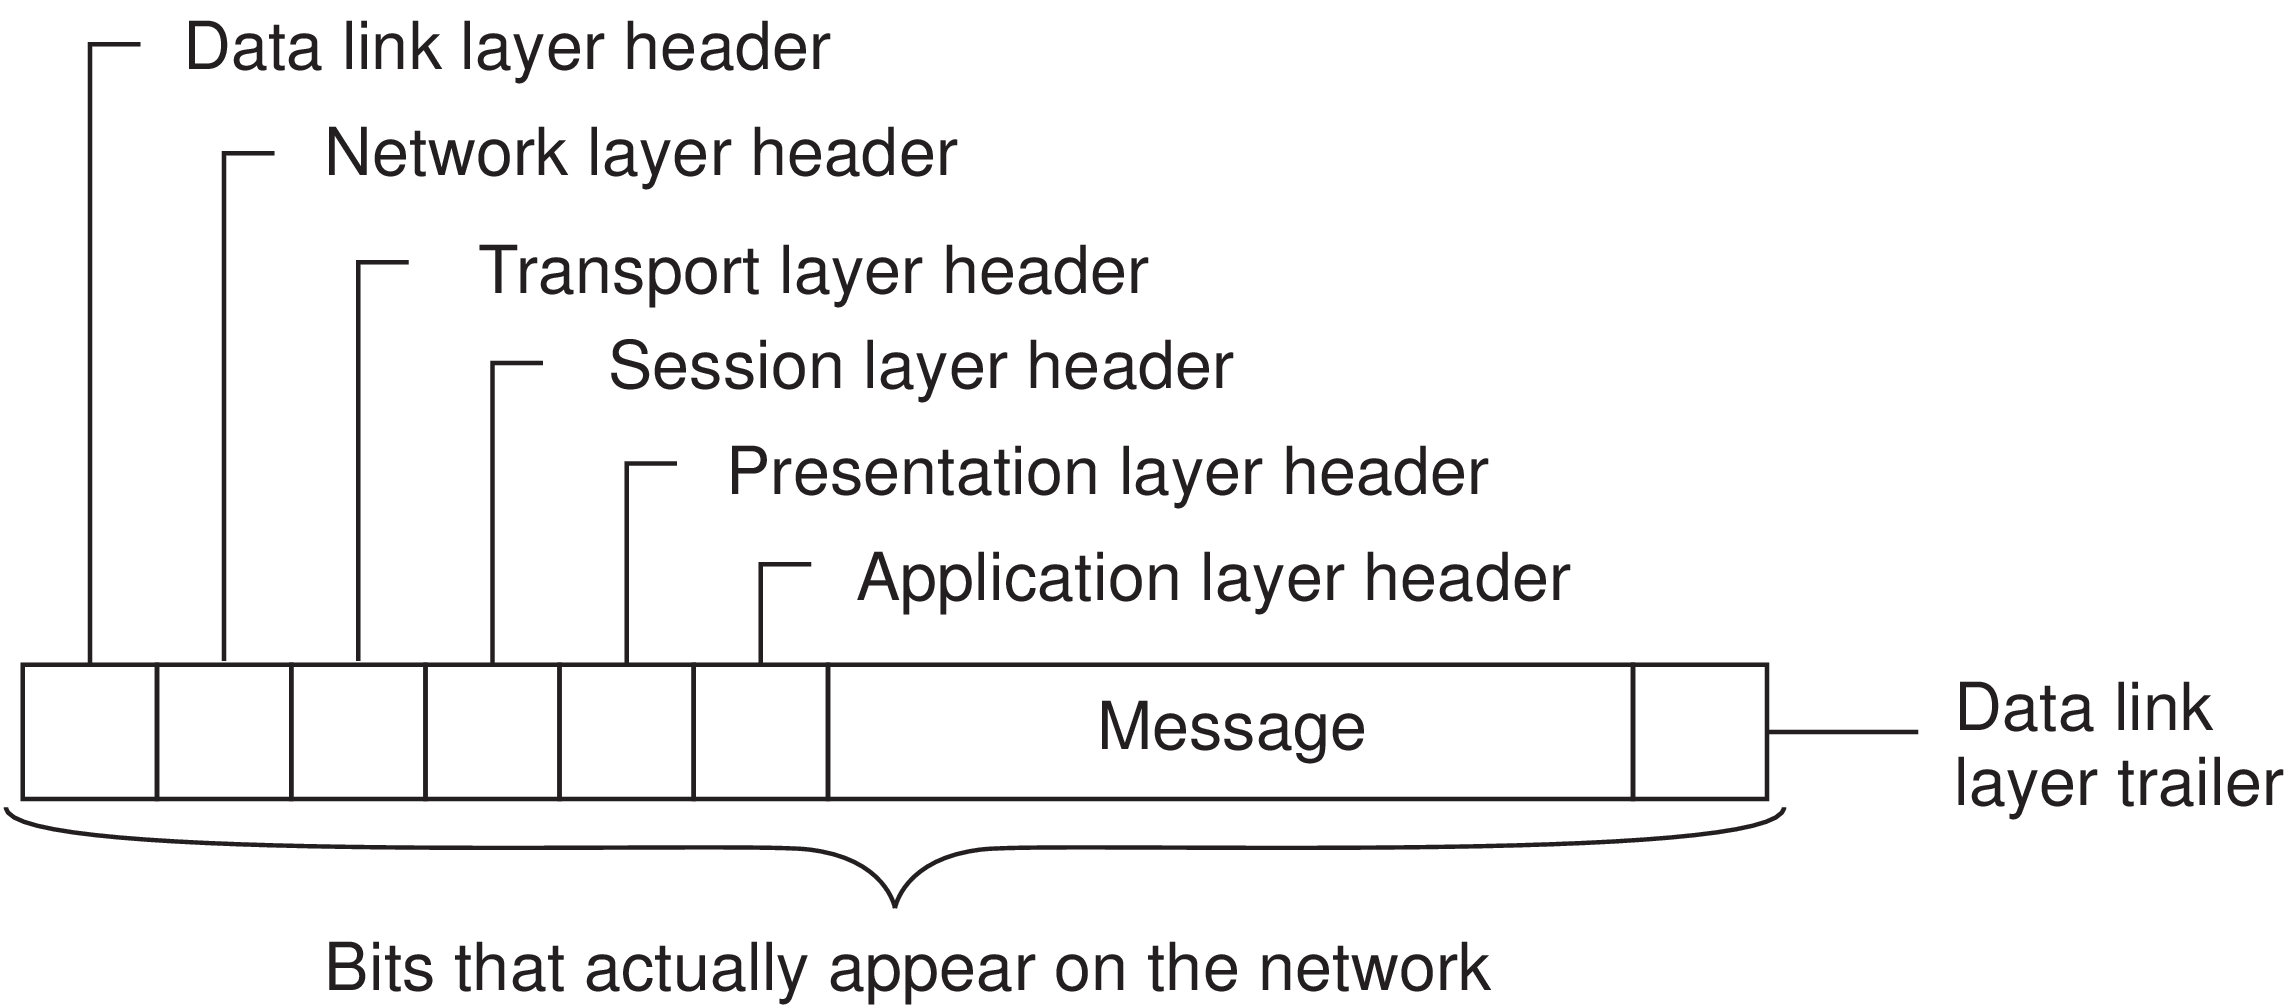
\includegraphics[width=0.95\textwidth]{images/osi_message.png}

\end{frame}

%% --------------------------------------------------------

\begin{frame}{Modelo TCP/IP}

O modelo OSI é um modelo de referência que nos ajuda a \textit{entender} como redes funcionam

\vspace{1cm}

Já o modelo TCP/IP apresenta o modelo que realmente funciona no mundo real
\begin{itemize}
    \item Baseada nos protocolos TCP e IP
    \item É a maneira como a Internet está implementada e organizada
\end{itemize}

\end{frame}

%% --------------------------------------------------------

\begin{frame}{TCP/IP \textit{vs} OSI}

\vspace{0.5cm}

\centering 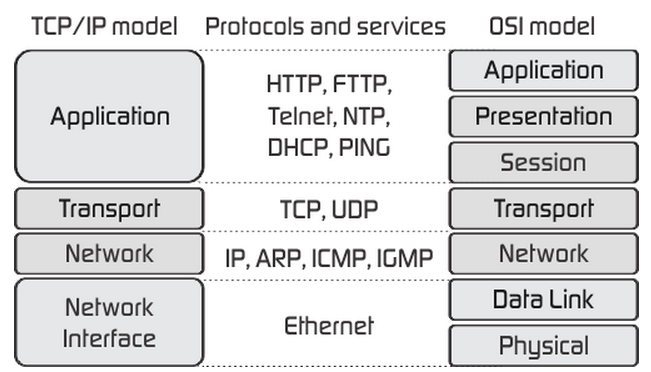
\includegraphics[width=\textwidth]{images/protocolos.png}

\end{frame}

%% --------------------------------------------------------

\begin{frame}{Protocolos de \textit{middleware}}

Um \textit{middleware} está localizado logicamente na camada de aplicação do modelo TCP/IP


Um protoclo de \textit{middleware} deve fornecer uma interface transparente para as aplicações trabalharem e trocarem mensagens
\begin{itemize}
    \item Responsável por coordenar todo o sistema distribuído
\end{itemize}

\end{frame}

%% --------------------------------------------------------

\begin{frame}{Protocolos de \textit{middleware}}

\vspace{0.5cm}

\centering 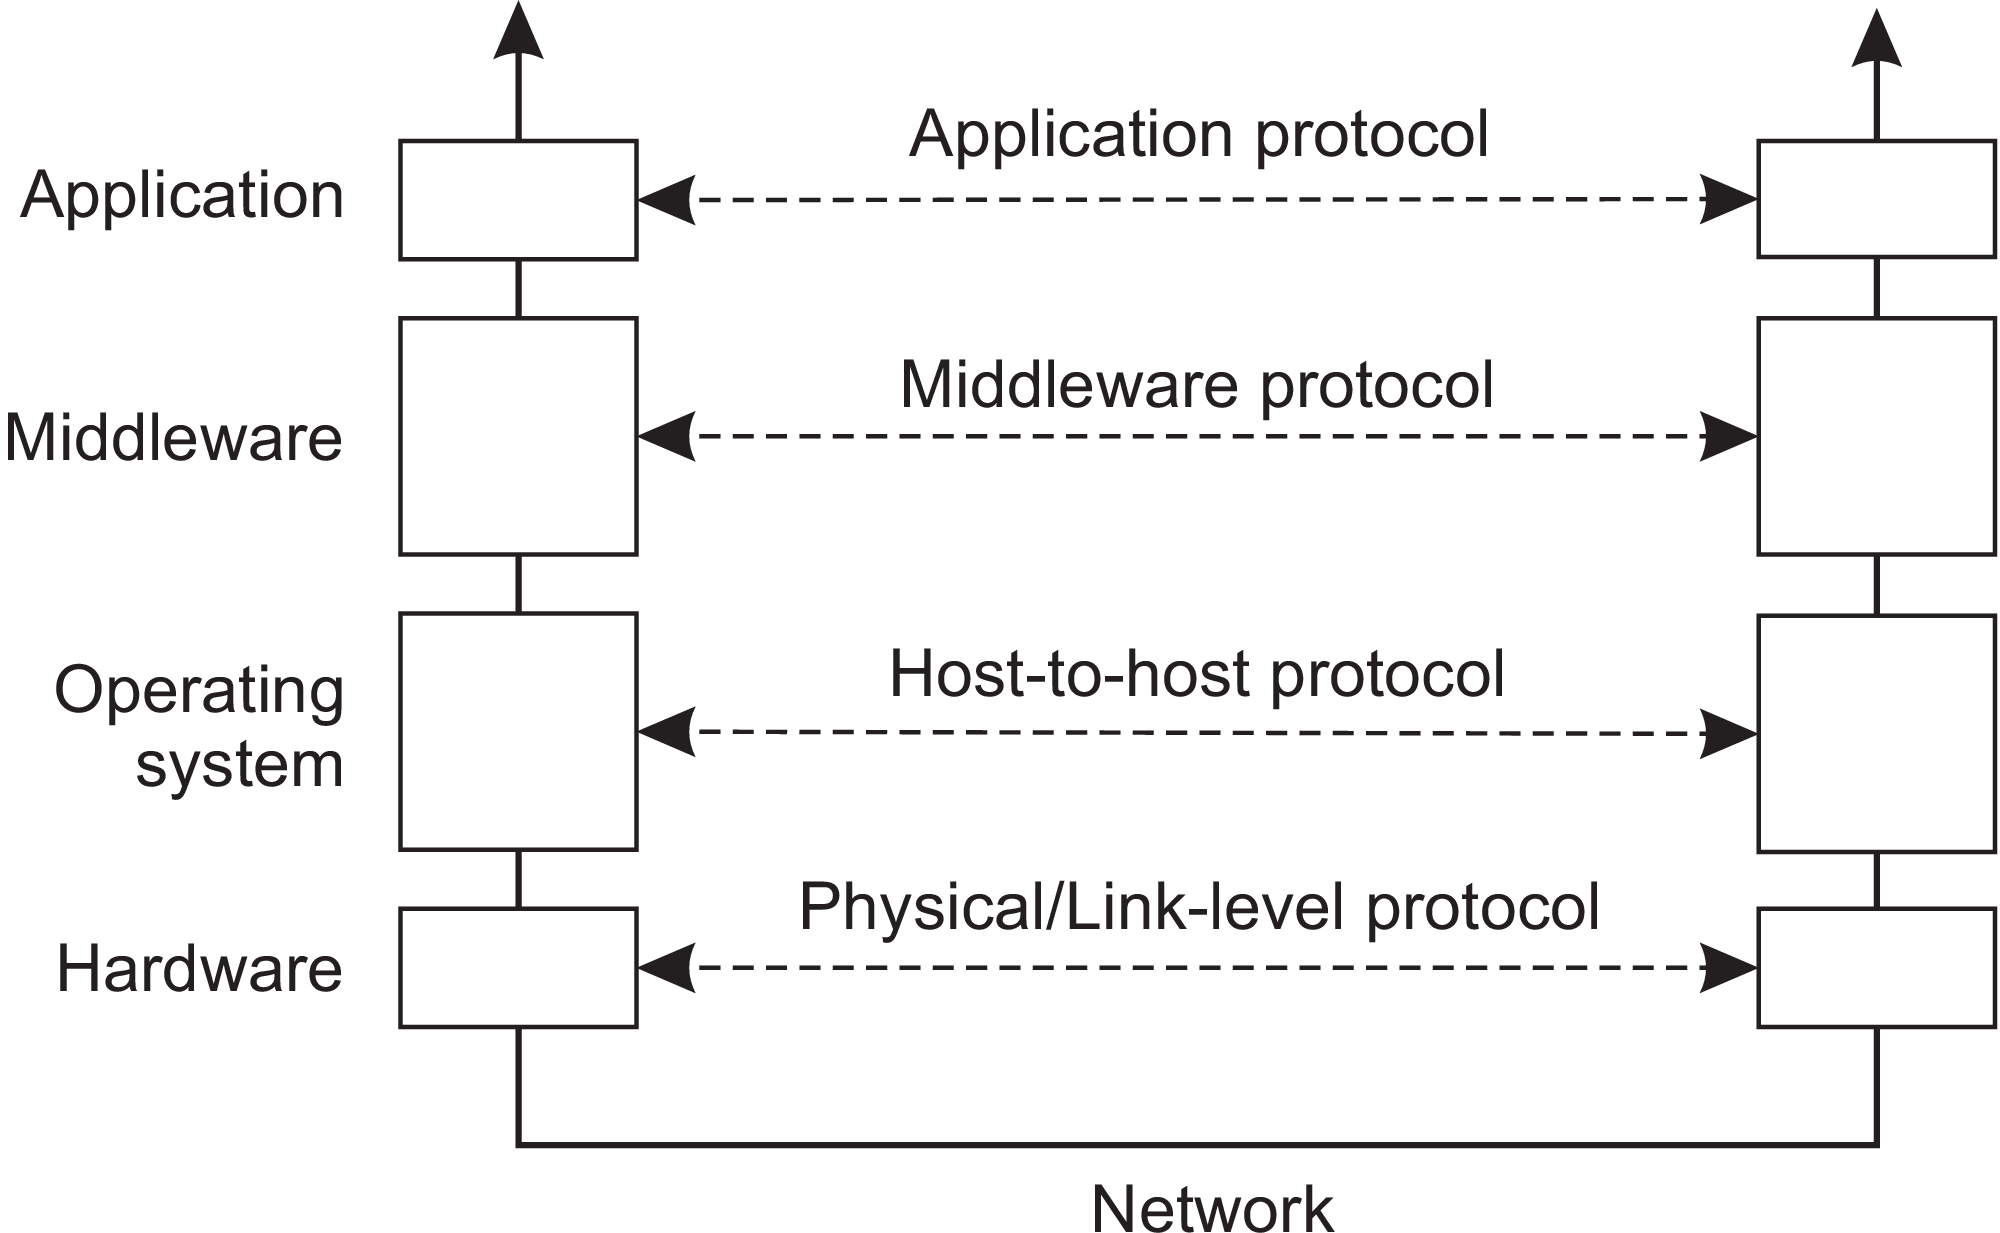
\includegraphics[width=\textwidth]{images/osi_adapted.png}

\end{frame}

%% --------------------------------------------------------

\begin{frame}{Tipos de comunicação}

O restante de nossas aulas deverá focar em protocolos de comunicação oferecidos por \textit{middlewares}
\begin{itemize}
    \item Oferece serviços de comunicação para as aplicações (componentes)
\end{itemize}

Um \textit{middleware} implementa dois diferentes tipos de comunicação
\begin{itemize}
    \item Persistente
    \item Transiente
\end{itemize}

Estas comunicações também podem ser de dois tipos
\begin{itemize}
    \item Síncronas
    \item Assíncronas
\end{itemize}
\end{frame}

%% --------------------------------------------------------

\begin{frame}{Modelos de persistência de mensagens}

Comunicação persistente
\begin{itemize}
    \item Mensagens enviadas por aplicações são armazenadas pelo \textit{middleware}
    \item Deve ser replicada (caso necessário)
    \item Mensagem fica armazenada até que não seja mais necessária
    \begin{itemize}
        \item Então, pode ser deletada
    \end{itemize}
\end{itemize}

Comunicação transiente
\begin{itemize}
    \item Mensagem é armazenada no \textit{middleware} enquanto as aplicações estão rodando
    \begin{itemize}
        \item Aplicação remetente
        \item Aplicação desninatária
    \end{itemize}
    \item Normalmente, protocolos da camada de transmissão utilizam comunicação transiente
\end{itemize}
\end{frame}

%% --------------------------------------------------------

\begin{frame}{Síncronia de mensagens}

Similar aos conceitos que vimos em arquiteturas de sistemas distribuídos

\vspace{0.5cm}

Comunicação síncrona
\begin{itemize}
    \item Processo remetente fica bloqueado até receber uma resposta
\end{itemize}

\vspace{0.5cm}
Comunicação assíncrona
\begin{itemize}
    \item Processo remetente não é bloqueado até receber resposta
\end{itemize}

\vspace{0.5cm}

Comunicação transiente + mensagens síncronas \textcolor{sthlmDarkBlue}{$\rightarrow$} RPC
\begin{itemize}
    \item Próxima aula
\end{itemize}
\end{frame}

\end{document}
